\begin{figure}[htbp]
\centering
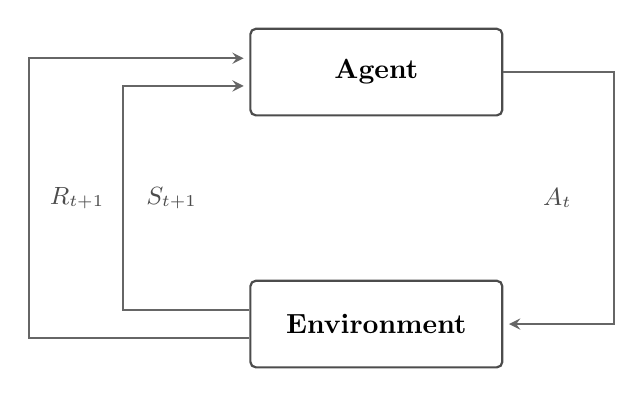
\begin{tikzpicture}[
    box/.style={draw=black!70, thick, minimum width=3.2cm,
                minimum height=1.1cm, font=\normalsize\bfseries,
                rounded corners=2pt},
    arr/.style={->, thick, >=stealth, black!60, shorten >=2pt},
    lbl/.style={font=\small, text=black!70},
]

% Nodes
\node[box] (agent) at (0, 3.2) {Agent};
\node[box] (env)   at (0, 0)   {Environment};

% Action: agent -> environment (right side)
\draw[arr] (agent.east) -- ++(1.4, 0) |- (env.east);
\node[lbl] at (2.3, 1.6) {$A_t$};

% Reward: environment -> agent (outer left)
\draw[arr] ([yshift=-5pt]env.west) -- ++(-2.8, 0)
    |- ([yshift=5pt]agent.west);

% State: environment -> agent (inner left)
\draw[arr] ([yshift=5pt]env.west) -- ++(-1.6, 0)
    |- ([yshift=-5pt]agent.west);

% Labels between the two vertical segments
\node[lbl] at (-3.8, 1.6) {$R_{t+1}$};
\node[lbl] at (-2.6, 1.6) {$S_{t+1}$};

\end{tikzpicture}
\caption{The agent--environment loop. At each time step the agent
  observes state $S_t$, selects action $A_t$, and receives reward
  $R_{t+1}$ as the environment transitions to $S_{t+1}$.}
\label{fig:mdp-loop}
\end{figure}
